\documentclass{standalone}

% graphics
\usepackage{tikz}
\usepackage{pgfplots}
\usepackage{siunitx}

\begin{document}

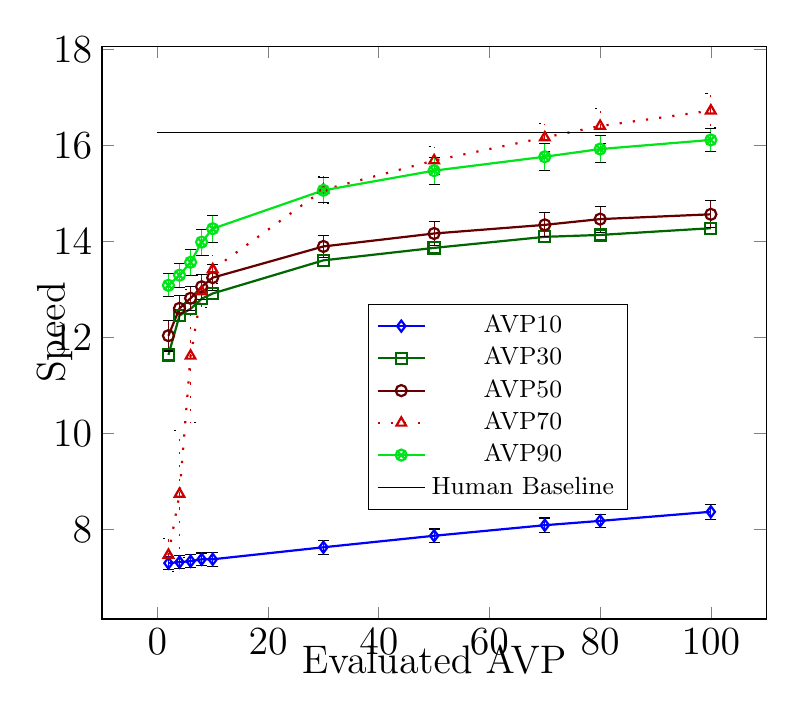
\begin{tikzpicture}[scale=1]
  \pgfplotsset{
      scale only axis,
      every x tick label/.append style={font=\Large},
      every y tick label/.append style={font=\Large},
	legend style={at={(0.4,0.55)},anchor=north west}
  }

\begin{axis}[
    legend style={font=\small},
	ylabel={\Large Speed},
	x label style={at={(axis description cs:0.5,-0.03)},anchor=north},
	y label style={at={(axis description cs:-0.030,0.5)}, anchor=south},
	xlabel={\Large Evaluated AVP},
]


% trained on avp=10 
% dashdotdotted,
\addplot[mark=diamond, thick, mark options={solid, fill=blue!40, mark size=2 pt}, draw=blue, error bars/.cd, y dir=both, y explicit] table [x=a, y=b, y error=c] {
a	b   	c
2 7.30 0.14
4 7.32 0.14
6 7.34 0.14
8 7.38 0.13
10 7.38 0.15
30 7.63 0.15
50 7.87 0.14
70 8.09 0.15
80 8.18 0.13
100 8.37 0.16
};
\label{AVP10}

% trained on avp=30
% error bars/.cd, y dir=both, y explicit,
\addplot[mark=square, thick, mark options={solid, fill=green!60, mark size=2 pt}, draw=black!60!green] table [x=a, y=b] {
a	b   	c
2 11.64 0.32
4 12.46 0.25
6 12.60 0.25
8 12.81 0.24
10 12.92 0.25
30 13.61 0.25
50 13.87 0.23
70 14.10 0.27
80 14.14 0.26
100 14.28 0.25
};
\label{AVP30}  

%densely dashed, 
\addplot[mark=o, thick, mark options={solid, fill=black!60!red, mark size=2pt}, draw=black!60!red, error bars/.cd, y dir=both, y explicit] table [x=a, y=b, y error=c] {
a	b   	c
2 12.04 0.32
4 12.61 0.26
6 12.82 0.25
8 13.06 0.26
10 13.25 0.27
30 13.90 0.23
50 14.17 0.25
70 14.35 0.25
80 14.47 0.27
100 14.57 0.28
};
\label{AVP50}

%densely dashed, 
\addplot[mark=triangle, thick, loosely dotted, mark options={solid, fill=red!60, mark size=2pt}, draw=black!20!red, error bars/.cd, y dir=both, y explicit] table [x=a, y=b, y error=c] {
a	b   	c
2 7.47 0.34
4 8.74 1.33
6 11.62 1.39
8 12.96 0.34
10 13.42 0.30
30 15.08 0.28
50 15.69 0.29
70 16.17 0.29
80 16.41 0.37
100 16.73 0.35
};
\label{AVP70}

%densely dashed, 
\addplot[mark=otimes, thick, mark options={solid, fill=red!60, mark size=2pt},
draw=blue!10!green, error bars/.cd, y dir=both, y explicit] table [x=a, y=b, y error=c] {
a	b   	c
2 13.09 0.24
4 13.30 0.25
6 13.57 0.27
8 13.99 0.27
10 14.27 0.28
30 15.07 0.26
50 15.48 0.28
70 15.77 0.28
80 15.93 0.28
100 16.12 0.24
};
\label{AVP90}


%%densely dashed, 
%\addplot[mark=otimes, thick, mark options={solid, fill=blue!60, mark size=2pt},
%draw=blue!10!red, error bars/.cd, y dir=both, y explicit] table [x=a, y=b, y error=c] {
%a	b   	c
%2 7.26 0.15
%4 7.24 0.15
%6 7.27 0.15
%8 7.30 0.18
%10 7.34 0.18
%20 7.55 0.17
%30 7.91 0.29
%40 8.41 0.44
%50 9.19 0.69
%60 10.73 0.76
%70 11.74 0.68
%80 12.37 0.67
%100 13.57 0.64 
%};
%\label{linearPPO}


\addplot[mark=none, black, samples=200] coordinates {(0,16.27) (100,16.27)};{};\label{Baseline}

\addlegendimage{/pgfplots/refstyle=AVP10}
\addlegendentry{AVP10}

\addlegendimage{/pgfplots/refstyle=AVP30}
\addlegendentry{AVP30}

\addlegendimage{/pgfplots/refstyle=AVP50}
\addlegendentry{AVP50}

\addlegendimage{/pgfplots/refstyle=AVP70}
\addlegendentry{AVP70}

\addlegendimage{/pgfplots/refstyle=AVP90}
\addlegendentry{AVP90}

%\addlegendimage{/pgfplots/refstyle=linearPPO}
%\addlegendentry{linearPPOAVP10}

\addlegendimage{/pgfplots/refstyle=Baseline}
\addlegendentry{Human Baseline}




\end{axis}
\end{tikzpicture}

\end{document}

